\section{Kiến trúc của IPFS}

\subsection{Đối tượng IPFS}

Một đối tượng IPFS (IPFS Object hay còn được ký hiệu là IPLD) là một cấu trúc dữ liệu với hai trường:
\begin{itemize}
    \item \texttt{Data}: Dữ liệu nhị phân không có cấu trúc có kích thước nhỏ hơn $256\mathrm{kB}$.
    \item \texttt{Links}: Chứa các liên kết (\texttt{Link}) đến các đối tượng IPFS khác.
\end{itemize}

Cấu trúc của \texttt{Link} gồm ba trường:
\begin{itemize}
    \item \texttt{Name}: Tên của liên kết.
    \item \texttt{Hash}: Hàm băm của đối tượng IPFS được liên kết tới.
    \item \texttt{Size}: Kích thước tích luỹ của đối tượng IPFS được liên kết tới, bao gồm cả các liên kết sau đó nữa.
\end{itemize}
Trong đó, trường \texttt{Size} chủ yếu được sử dụng cho việc tối ưu hoá mạng P2P.

\subsection{Merkle-DAG}

DAG (Directed Acyclic Graph) là một dạng đồ thị có hướng, trong đó mỗi nút sẽ liên kết với các nút khác và không cho phép tạo thành chu trình có hướng. Một nút mà không là con của một nút nào khác trong đồ thị được gọi là nút gốc.\\

Merkle-DAG là một DAG trong đó mỗi nút có một định danh (identity hay id) là kết quả của việc mã hoá nội dung của nút đó. Điều này mang lại một số lưu ý:
\begin{itemize}
    \item Các nút con phải được sinh trước thì các nút cha mới có id để liên kết tới.
    \item Mỗi nút trong Merkle-DAG là một nút gốc của một Merkle-DAG con nào đó.
    \item Các nút trong Merkle-DAG là không thể thay đổi. Bất kỳ thay đổi nào trong một nút sẽ làm thay đổi id của nút đó, và ảnh hưởng đến tất cả các nút khác.
\end{itemize}

\begin{figure}[!ht]
    \centering
    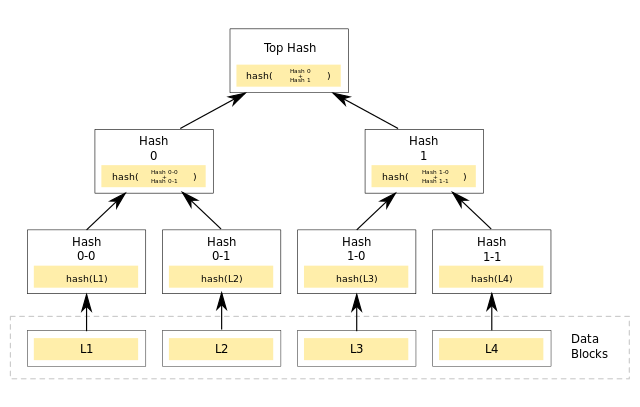
\includegraphics[width=250px]{anh/ipfs/merkle-tree.png}
    \caption{Ví dụ về một Merkle-DAG.}
\end{figure}

\subsection{Hệ thống tập tin}

IPFS dễ dàng biểu diễn một hệ thống các tập tin và thư mục.

\subsubsection*{Các tập tin nhỏ}

Một tập tin nhỏ được định nghĩa có kích thước nhỏ hơn $256\mathrm{kB}$, được biểu thị bằng một đối tượng IPFS với trường \texttt{Data} chứa nội dung của nó và trường \texttt{Links} là một danh sách rỗng.\\

Do tên tập tin không phải là một phần của đối tượng IPFS nên nếu có hai tập tin có cùng nội dung, chúng sẽ được biểu diễn bởi cùng một đối tượng IPFS.

\subsubsection*{Các tập tin lớn}

Một tập tin lớn được định nghĩa có kích thước không dưới $256\mathrm{kB}$, được biểu thị bởi một Merkle-DAG của các đối tượng IPFS sao cho mỗi đối tượng có kích thước dữ liệu nhỏ hơn $256\mathrm{kB}$.\\
